\documentclass[aps,prl,preprint
,superscriptaddress]{revtex4-1}
\newcommand{\SSC}{S/S_{c}}
\newcommand{\mnras}{Monthly Notices of the Royal Astronomical Society}
\newcommand{\apjs}{The Astrophysical Journal Supplement Series}
\usepackage{graphicx}
\usepackage{amssymb}
\usepackage{amsmath}

% You should use BibTeX and apsrev.bst for references
% Choosing a journal automatically selects the correct APS
% BibTeX style file (bst file), so only uncomment the line
% below if necessary.
%\bibliographystyle{apsrev4-1}

\newcommand\Beq{\begin{eqnarray}} 
\newcommand\Eeq{\end{eqnarray}}

\newcommand{\Eq}[1]{Eq.~(\ref{#1})}
\newcommand{\Eqs}[2]{Eqs.~(\ref{#1})--(\ref{#2})}
\newcommand{\eq}[1]{eq.~(\ref{#1})}
\newcommand{\eqs}[2]{eqs.~(\ref{#1})--(\ref{#2})}

\newcommand{\Prob}[2]{\mathbb{P}[\, #1 \, | \, #2 \, ] }
\newcommand{\Pro}[1]{\mathbb{P}[\, #1 \, ] }

\newcommand{\inv}[1]{\frac{1}{#1}}
\newcommand{\pd}[1]{\partial_{#1}}

\newcommand{\Reyn}{\mathrm{Re}}
\newcommand{\Reym}{\mathrm{Rm}}
\newcommand{\Ra}{R}
\newcommand{\Ve}{\mbox{\textit{Ve}}}
\newcommand{\eps}{\varepsilon}
\newcommand{\del}{\delta}
\newcommand{\e}[1]{\eps^{#1}}
\newcommand{\f}{2\Omega}

\newcommand{\n}{\hat{n}}


\newcommand{\dat}{\cdot}
\newcommand{\dd}[1]{\,\mathrm{d}{#1}}
\newcommand{\cc}{\mathrm{c.c.}}
\renewcommand{\vec}[1]{\boldsymbol{#1}}
\newcommand{\grad}{\nabla}
\renewcommand{\div}{\nabla \dat}
\newcommand{\Tr}{\text{Tr}}


\newcommand{\pren}[1]{ \left(#1\right) }
\newcommand{\brac}[1]{\left[\,#1\,\right]}

\newcommand{\ave}[1]{\big<#1\big>}

\renewcommand{\l}{\ell}

\newcommand{\txt}[1]{\quad \text{#1} \quad }

\begin{document}

% Use the \preprint command to place your local institutional report
% number in the upper righthand corner of the title page in preprint mode.
% Multiple \preprint commands are allowed.
% Use the 'preprintnumbers' class option to override journal defaults
% to display numbers if necessary
%\preprint{}

%Title of paper
\title{Supplemental Information for: The Magnetorotational Instability Prefers Three Dimensions}

\maketitle
\section{Numerical Methods and Resolution Studies}
\label{sec:methods}

For both the ideal and non-ideal MHD equations, we solve the eigenvalue problem in the $x$ direction using the \texttt{EigenValueProblem} solver in \emph{Dedalus} for a grid of $N_y \times N_z$ modes in the $y$ and $z$ directions.
For most of our runs, we use a targeted, sparse eigenvalue solver to find the 15 modes closest to a guess for the maximum growth rate.
In run 3, we have confirmed that dense solvers retrieve identical results.
For nearly ideal runs, we use the ideal 2D growth rate as input for the smallest $k_y > 0$ mode at each $k_z$ and then use the output from each previous $k_y$ as an input guess for the next mode.
For those runs that have significant $\eta$, we instead use a dense solve for the $k_y = 0$ modes and then step forward in $k_y$ at each $k_z$ as before.
Our solver is embarrassingly parallelized over the $k_z$ modes.
For the spectrum in figure 1 of the main text, we used a dense eigenvalue solver at $(k_y^{max},k_z^{max})$ for $\SSC= 1.02$.

In order to ensure our results are converged, we have repeated runs at $n_x=256$ Chebyshev modes as well as doubling the number of modes in $y$ and $z$.

\begin{tabular}{cccccccccccccc}
\textbf{Run} & \textbf{$\SSC$} & \textbf{$\nu$} & \textbf{$\eta$} & \textbf{$q$} & \textbf{$N_x$} & \textbf{$N_{k_y}$} & \textbf{$N_{k_z}$} & \textbf{Sparse/Dense}& \\
1  &   1.02 & $10^{-5}$ & $10^{-5}$ & 0.75 & 128 & 200 & 200 & sparse & resolution study\\
2  &   1.02 & $10^{-5}$ & $10^{-5}$ & 0.75 & 256 & 200 & 200 & sparse & \\
3  &   1.02 & $10^{-5}$ & $10^{-5}$ & 0.75 & 128 & 200 & 200 & dense  & \\
4  &   1.02 & $10^{-5}$ & $10^{-5}$ & 0.75 & 128 & 512 & 512 & sparse & \\
5  &   1.02 & $10^{-5}$ & $10^{-5}$ & 0.75 & 128 & 100 & 100 & sparse & \\
6  &   0.2  & $10^{-5}$ & $10^{-5}$ & 0.75 & 128 & 200 & 200 & sparse & $\SSC$ variation\\
7  &   0.3  & $10^{-5}$ & $10^{-5}$ & 0.75 & 128 & 200 & 200 & sparse & \\
8  &   0.4  & $10^{-5}$ & $10^{-5}$ & 0.75 & 128 & 200 & 200 & sparse & \\
9  &   0.5  & $10^{-5}$ & $10^{-5}$ & 0.75 & 128 & 200 & 200 & sparse & \\
10 &   0.64 & $10^{-5}$ & $10^{-5}$ & 0.75 & 128 & 200 & 200 & sparse & \\
11 & 1.020  & $10^{-5}$ & $10^{-5}$ & 0.75 & 128 & 200 & 200 & sparse & \\
12 & 1.44   & $10^{-5}$ & $10^{-5}$ & 0.75 & 128 & 200 & 200 & sparse & \\
13 & 1.75   & $10^{-5}$ & $10^{-5}$ & 0.75 & 128 & 200 & 200 & sparse & \\
14 & 1.891  & $10^{-5}$ & $10^{-5}$ & 0.75 & 128 & 200 & 200 & sparse & \\
15 & 2.     & $10^{-5}$ & $10^{-5}$ & 0.75 & 128 & 200 & 200 & sparse & \\
16 & 2.01   & $10^{-5}$ & $10^{-5}$ & 0.75 & 128 & 200 & 200 & sparse & \\
17 & 2.015  & $10^{-5}$ & $10^{-5}$ & 0.75 & 128 & 200 & 200 & sparse & \\
18 & 2.031  & $10^{-5}$ & $10^{-5}$ & 0.75 & 128 & 200 & 200 & sparse & \\
19 & 2.05   & $10^{-5}$ & $10^{-5}$ & 0.75 & 128 & 200 & 200 & sparse & \\
20 & 2.1    & $10^{-5}$ & $10^{-5}$ & 0.75 & 128 & 200 & 200 & sparse & \\
21 & 2.25   & $10^{-5}$ & $10^{-5}$ & 0.75 & 128 & 200 & 200 & sparse & \\
22 & 2.5    & $10^{-5}$ & $10^{-5}$ & 0.75 & 128 & 200 & 200 & sparse & \\
23 & 4      & $10^{-5}$ & $10^{-5}$ & 0.75 & 128 & 200 & 200 & sparse & \\
24 & 1.02   & $10^{-6}$ & $10^{-6}$ & 0.75 & 128 & 200 & 200 & sparse & Reynolds number study\\
25 & 1.02   & $10^{-4}$ & $10^{-4}$ & 0.75 & 128 & 200 & 200 & sparse & \\
26 & 1.02   & $10^{-3}$ & $10^{-3}$ & 0.75 & 128 & 200 & 200 & sparse & \\
27 & 1.02   & $10^{-2}$ & $10^{-2}$ & 0.75 & 128 & 200 & 200 & sparse & \\
28 & 1.02   & $10^{-5}$ & $10^{-5}$ & 0.1  & 128 & 200 & 200 & sparse & Low Rossby\\ 
29 & 1.02   & $10^{-6}$ & $10^{-2}$ & 0.1  & 128 & 200 & 200 & sparse & Liquid metal case\\ 
\end{tabular}
%\label{simulations}

\section{1st-order formulation of the dissipative equations}
\label{sec:formulation}

We formulate the system in terms of the 10 problem \texttt{variables} 
\Beq
X \ = \ \left[\,p,v_{x},v_{y},v_{z},\omega_{y},\omega_{z},b_{x},b_{y},b_{z},j_{xx}\,\right] \nonumber
\Eeq
As sting-based \texttt{substitutions} 
\Beq
``\omega_{x}" &=& ``\pd{y} v_{z} - \pd{z} v_{y}" \nonumber \\
``j_{x}" &=& ``\pd{y} b_{z} - \pd{z} b_{y}" \nonumber \\
``j_{y}" &=& ``\pd{z} b_{x} - \pd{x} b_{z}" \nonumber \\
``j_{z}" &=& ``\pd{x} b_{y} - \pd{y} b_{x}" \nonumber 
\Eeq
The expression for $\omega_{x},\,j_{x},\,j_{y},\,j_{z}$ are not legitimate variables that \textit{Dedalus} solves for. They are only short-hand aliases that mean literally the same thing as the expression on the right-hand side of the definition, which are defined strictly in terms of legitimate problem variables. 

We also define the following operator substitutions 
\Beq
``\pd{t} q" &=& ``\sigma q" \nonumber \\
``\pd{y} q" &=& ``i k_{y} q" \nonumber \\
``\pd{z} q" &=& ``i k_{z} q" \nonumber 
\Eeq
where $\sigma$ is the problem \texttt{eigenvalue}, and $k_{y},\,k_{z}$ are problem \texttt{parameters}, along with $f,\,S,\,B_{0},\, \nu,\, \eta$.

The system of \texttt{equations} is:
\Beq\label{u-eq}
\pd{x} v_{x} + \pd{y} v_{y} + \pd{z} v_{z}  &=& 0\\
\pd{t} v_{x} + S x \pd{y} v_{x} - f v_{y} + \pd{x} p - B_{0} \pd{z} b_{x}  + \nu ( \pd{y} \omega_{z} - \pd{z} \omega_{y}) &=& 0\\
\pd{t} v_{y} + S x \pd{y} v_{y} + (f+S) v_{x} + \pd{y} p - B_{0} \pd{z} b_{y} + \nu ( \pd{z} \omega_{x} - \pd{x} \omega_{z})&=& 0\label{v-eq} \\
\pd{t} v_{z} + S x \pd{y} v_{z} + \pd{z} p - B_{0} \pd{z} b_{z} + \nu ( \pd{x} \omega_{y} - \pd{y} \omega_{x})&=& 0 \\
\omega_{y} - \pd{z} v_{x} + \pd{x} v_{z} &=& 0 \\
\omega_{z} - \pd{x} v_{y} + \pd{y} v_{x} &=& 0 \\
\pd{x} b_{x} + \pd{y} b_{y} + \pd{z} b_{z}   &=& 0\\
\pd{t} b_{x} + S x \pd{y} b_{x} - B_{0} \pd{z} v_{x} + \eta ( \pd{y} j_{z} - \pd{z} j_{y})&=& 0\\
\pd{t} j_{x}  + S x \pd{y} j_{x}- \eta( \pd{x}j_{xx} + \pd{y}^{2} j_{x} + \pd{z}^{2} j_{x} )  - B_{0} \pd{z} \omega_{x} + S \pd{z} b_{x} &=& 0\\
j_{xx} - \pd{x} j_{x} &=& 0
\Eeq
We can see there are the same number of equations as variables, each equations has only 1st-order derivatives in $x$, and every variable has at least one $\pd{x}$. It appears (for example) that there are no $\pd{x}$ terms in the $b_{x}$ equation, but this due to the substitutions, 
\Beq
\pd{y} j_{z} - \pd{z} j_{y} =  \pd{y}(\pd{x} b_{y} - \pd{y} b_{x}) - \pd{z}(\pd{z} b_{x} - \pd{x} b_{z})  =  \pd{x}( \pd{y}b_{y} + \pd{z}b_{z}) - (\pd{y}^{2} + \pd{z}^{2})b_{x}.
\Eeq

The entire system is formulated and solved as a generalized eigenvalue problem with non-constant coefficients 
\Beq
\sigma \, M \cdot X + L_{0}(x) \cdot X + L_{1}\cdot \pd{x} X \ = \ 0
\Eeq
The system is 10th order because $L_{1}$ has full rank. We therefore impose the 10 \texttt{boundary conditions} 
\Beq
v_{x} \ = \ \omega_{y} \ = \ \omega_{z} \ = \ b_{x} \ = \ j_{xx} \ = \ 0 \quad \text{at} \quad x \ = \ \pm d/2
\Eeq
We could choose any other set of boundary conditions constructed out of a linearly independent combinations of the legitimate problem variables. We choose impenetrable stress-free and perfectly conducting because it agrees with the purely impenetrable conditions for an ideal calculation.

\section{Reynolds Number and Departure from Ideal MHD}
\label{sec:reyn}

In order to ensure that our calculations are probing the ideal MHD regime we are interested in, we have performed as series of runs (24-27) with the $\eta = \nu$ ranging from $10^{-6}$ to $10^{-2}$.
In our units, this is equivalent to varying the Reynolds and Magnetic Reynolds numbers $\Reyn = \Reym = 10^2 -- 10^6$.
Figure~\pageref{fig:reynolds} shows the growth rates at $\SSC=1.05$ for five values of $\Reyn = \Reym$.
For $\Reyn \gtrsim 10^4$, the maximum growth rate is located at the same position and the same growth rate; the unstable region expands, as expected.
This suggests that our results at $\Reyn = 10^5$ are reasonably close to ideal MHD for the purposes of understanding the MRI's preference for 3D modes near shear onset.
\begin{figure}[h!]
  \centering
  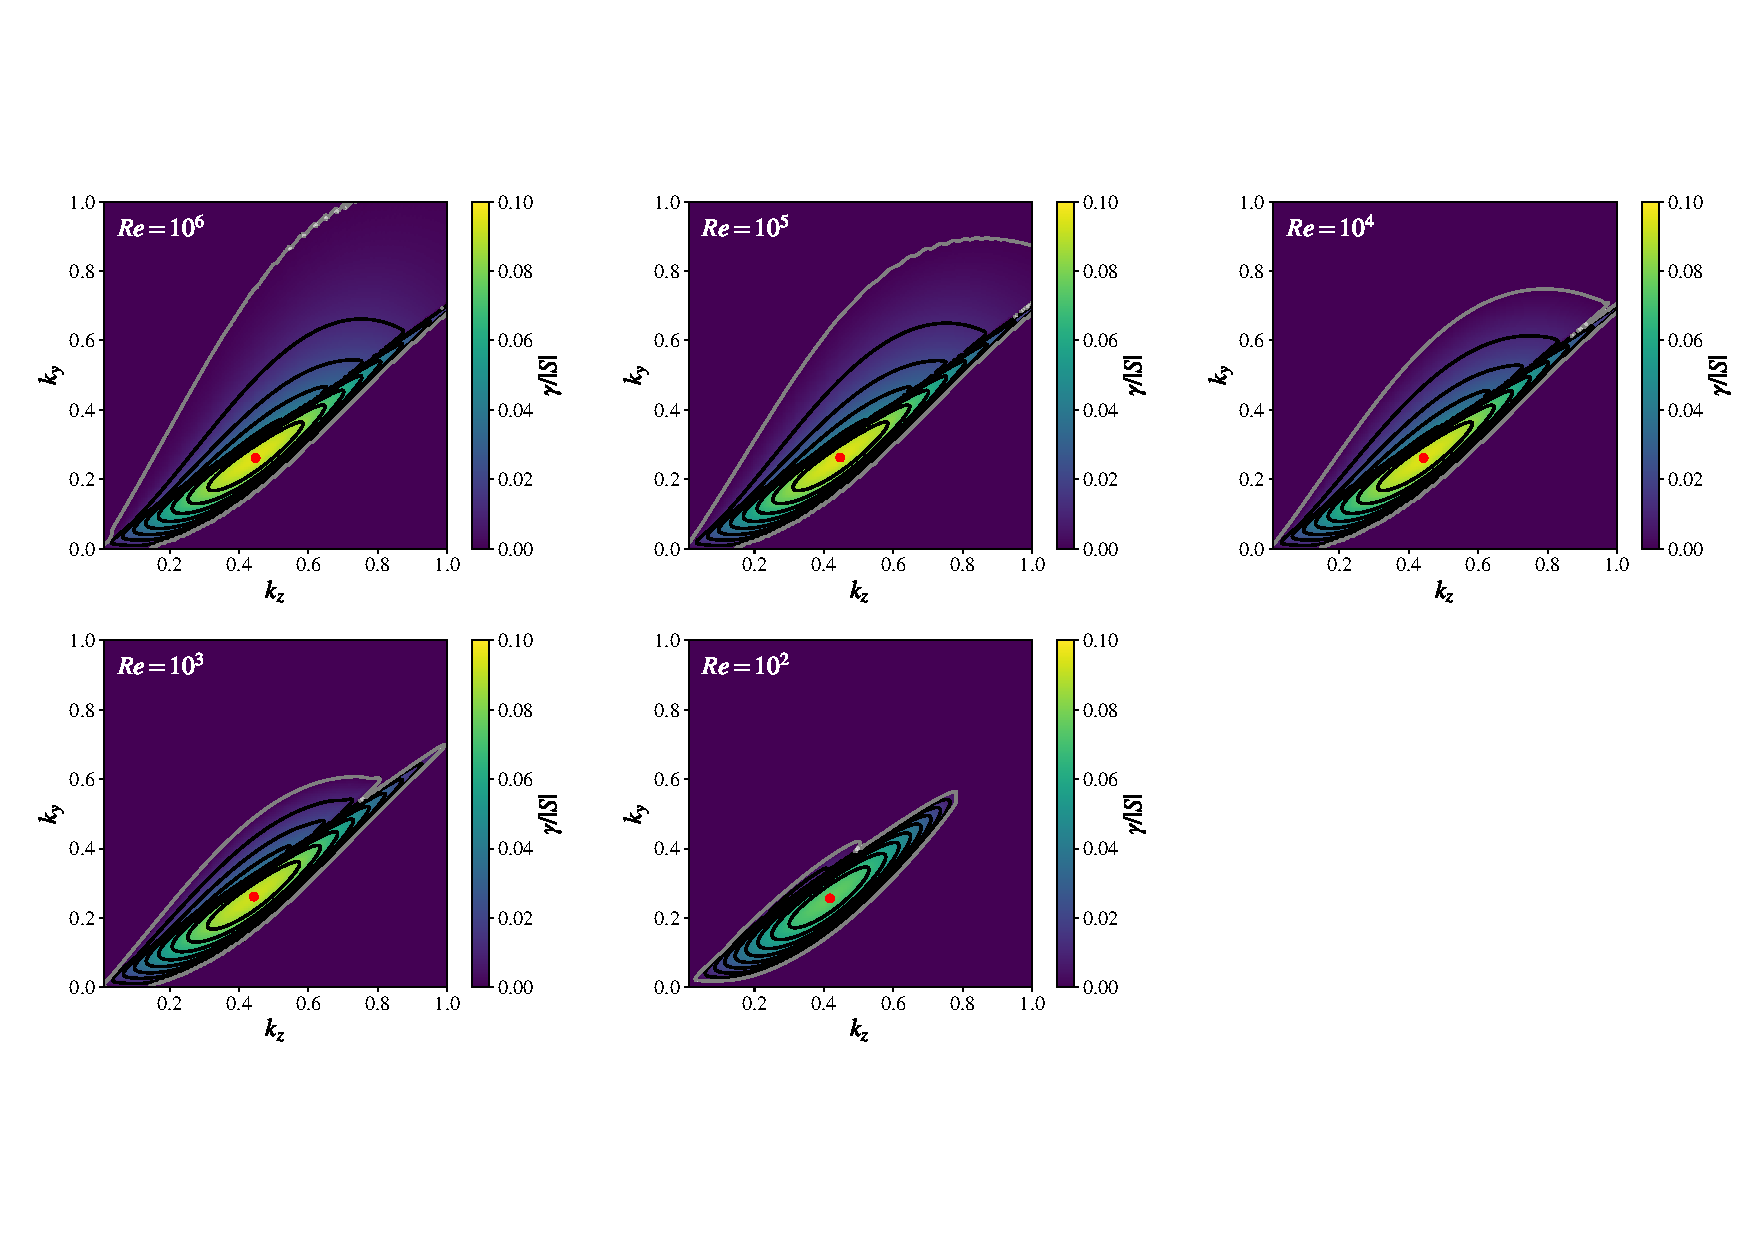
\includegraphics[width=\textwidth]{re_plots.pdf}
  \caption{Growth rates at $\SSC = 1.02$ for varying diffusivities. Note that the top three panels are essentially identical, suggesting that above $\Reyn \gtrsim 10^4$ we are reasonably close to ideal conditions.}
  \label{fig:reynolds}
\end{figure}

\section{Asymptotic Calculation}
\label{sec:asymp}
Here, we outline the asymptotic calculation for the leading order correction to the 2D growth rates in when accouting for three dimensional effects via finite $k_y$.
Define the domain as $ - d/2 < x < d/2$. Being in the rotating frame means the shear has no net
\Beq
\int_{-d/2}^{d/2} V_{y}(x) \text{d} x  \ = \ 0, \quad \implies  \quad V_{y}(x) \ = \ S\, x
\Eeq
The full linear ideal equations are:
\Beq\label{u-eq}
\pd{t} u + S x \pd{y} u - f v + \pd{x} p - B_{0} \pd{z} b_{x} &=& 0\\
\pd{t} v + S x \pd{y} v + (f+S) u + \pd{y} p - B_{0} \pd{z} b_{y} &=& 0\label{v-eq} \\
\pd{t} w + S x \pd{y} w + \pd{z} p - B_{0} \pd{z} b_{z} &=& 0 \\
\pd{x} u + \pd{y} v + \pd{z} w  &=& 0\\
\pd{t} b_{x} + S x \pd{y} b_{x} - B_{0} \pd{z} u &=& 0\\
\pd{t} b_{y} + S x \pd{y} b_{y} - B_{0} \pd{z} v - S b_{x}  &=& 0\\
\pd{t} b_{z} + S x \pd{y} b_{z} - B_{0} \pd{z} w &=& 0 \label{bz-eq}
\Eeq
All variables take the form
\Beq
g = \hat{G}(x) e^{ i ( \omega t + k z + \ell y ) } 
\Eeq
We solve the ideal eigenvalue problem in \textit{Dedalus} in the above formulation. To make analytical progress, define the frequency ``parameters'' 
\Beq
\omega_{S}(x) \ \equiv \ \omega + S x \ell, \quad \omega_{A}  \ \equiv \ B_{0} k.
\Eeq
We can use equations (\ref{v-eq}--\ref{bz-eq}) to find all amplitudes in terms of $\hat{U}(x)$ and $\hat{U}'(x)$. 
\Beq
\hat{V}(x) &=& \frac{i \left(\ell 
   \hat{U}'(x) + k^{2} \frac{ \left((f+S) \omega
   _S^2-S \omega _A^2\right)}{\omega _S
   \left(\omega _S^2-\omega _A^2\right)} \hat{U}(x)\right)}{k^2+\ell ^2} \\
\hat{W}(x) &=& \frac{i k \left(\hat{U}'(x)- \frac{ \left((f+S) \omega
   _S^2-S \omega _A^2\right)}{\omega _S
   \left(\omega _S^2-\omega _A^2\right)}  \ell 
   \hat{U}(x)\right)}{k^2+\ell ^2} \\
   \hat{P}(x) &=& \frac{i \left(\omega _A^2-\omega _S^2\right)
   \left(\hat{U}'(x) -  \ell \frac{ \left((f+S) \omega
   _S^2-S \omega _A^2\right)}{\omega _S
   \left(\omega _S^2-\omega _A^2\right)}
   \hat{U}(x)\right)}{\left(k^2+\ell ^2\right)
   \omega _S} \\
   \hat{B}_{x}(x) &=& \frac{\omega _A \hat{U}(x)}{\omega _S} \\
   \hat{B}_{y}(x) &=&\frac{\omega _A \hat{V}(x)}{\omega _S} -\frac{i S \omega _A \hat{U}(x)}{\omega _S^2} \\
   \hat{B}_{z}(x) &=& \frac{\omega _A \hat{W}(x)}{\omega _S}
   \Eeq
Substitute everything into equation (\ref{u-eq}) to get a second-order equation for $\hat{U}(x)$ of the general form 
\Beq
\alpha(x) \hat{U}''(x) + \beta(x) \hat{U}'(x) + \gamma(x) \hat{U}(x) \ = \ 0
\Eeq
where
\Beq
\alpha(x) &=& \omega _S^2-\omega _A^2 \\ 
   \beta(x) &=& \frac{2 S \ell  \omega _A^2}{\omega _S} \\
   \gamma(x) &=& \omega _A^2 \left(\frac{f^2 k^2}{\omega
   _S^2-\omega _A^2}-\frac{2 S^2 \ell
   ^2}{\omega _S^2}+k^2+\ell ^2\right)+f k^2
   (f+S)-\left(k^2+\ell ^2\right) \omega _S^2
\Eeq


We can eliminate the first-order term via
\Beq
\hat{U}(x) \ = \ \chi(x) \psi(x) \quad \text{where} \quad \chi'(x) \  = \ -\frac{\beta (x) \chi (x)}{2 \alpha (x)}
\Eeq
\Beq
-\psi''(x) + \Phi(x) \psi(x) \ = \ 0 \label{Schr-eq}
\Eeq
\Beq
\Phi(x)  \ = \ \frac{-2 \beta (x) \alpha '(x)+2 \alpha (x)
   \left(\beta '(x)-2 \gamma (x)\right)+\beta
   (x)^2}{4 \alpha (x)^2}
\Eeq
Putting everything together 
\Beq
\Phi(x) \ = \ \frac{S  \left(f k^2-S \ell
   ^2\right) \omega _A^2 -f k^2 (f+S) \omega
   _S^2}{\left(\omega _A^2-\omega
   _S^2\right){}^2} + k^{2} + \ell^{2}
\Eeq
If $\omega_{S}=-i \gamma+Sx\ell$, with $Re(\gamma)\neq0$ then the denominator of $\Phi(x)$ cannot vanish. 
We want to solve the Schr\"{o}dinger-type equation~(\ref{Schr-eq}) with the boundary conditions 
\Beq
\psi(x=\pm d/2) = 0.
\Eeq
We solve perturbatively near the critical values for the 2D  instability. We rescale each parameters in terms of a bookkeeping parameter, $\eps$.
\Beq
S  \ \to \  - \frac{\pi ^2 B_{0}^2}{d^2 f} ( 1 + \eps^{2} R), \quad \omega \ \to \ \eps^{2} \omega , \quad k \ \to \ \eps k, \quad \ell \ \to \ \eps^{2} \ell
\Eeq 
Also 
\Beq
q  \ \equiv  \ \frac{\pi ^2 B_{0}^2}{d^2 f^{2}}
\Eeq
Expanding to $\mathcal{O}(\eps^{2})$, 
\Beq
\Phi(x) \ = \ \frac{\pi^{2}}{d^{2}} + \eps^{2} \frac{B_{0}^2 f^2 q \left(k^2 R+q
   \ell ^2\right) - B_{0}^4 k^4 +f^2 (q+1) (\omega -f q x \ell
   )^2  }{B_{0}^4 k^2}
\Eeq
For leading order 
\Beq
\psi_{0}''(x) + \frac{\pi^{2}}{d^{2}}  \psi_{0}(x) \ = \ 0  \quad \implies \quad \psi_{0}(x) \ = \ \cos(\pi x / d).
\Eeq
The next order is
\Beq
\psi_{2}''(x) + \frac{\pi^{2}}{d^{2}}  \psi_{2}(x) + \Phi_{2}(x)\psi_{0}(x)\ = \ 0.
\Eeq
The solvability condition for $\psi_{2}(x)$ is 
\Beq
\int_{-d/2}^{d/2} \Phi_{2}(x)\psi_{0}(x)^{2} \text{d} x \ = \ 0.
\Eeq
This implies 
\Beq
-\omega^{2} \ = \ \frac{q\,B_{0}^{2}}{(q+1)} \left[ k_z^2 \left(R-\frac{d^2}{\pi^{2}} k_z^2\right) \ + \ \frac{\left(6+\pi ^2\right) q+\pi
   ^2-6}{12 } \, k_{y}^{2}  \right] \ + \ ...
\Eeq


\end{document}
